\documentclass[oneside,hidelinks]{book}
\usepackage{anysize}
\usepackage{amsmath}
\usepackage{mathabx} 
\usepackage{hyperref}
\usepackage{graphicx}
\usepackage{xcolor}
\usepackage[font=small,skip=3pt]{caption}
\usepackage{lmodern}
\usepackage{listings,lstautogobble}
\usepackage{pdfpages}
\begin{document}
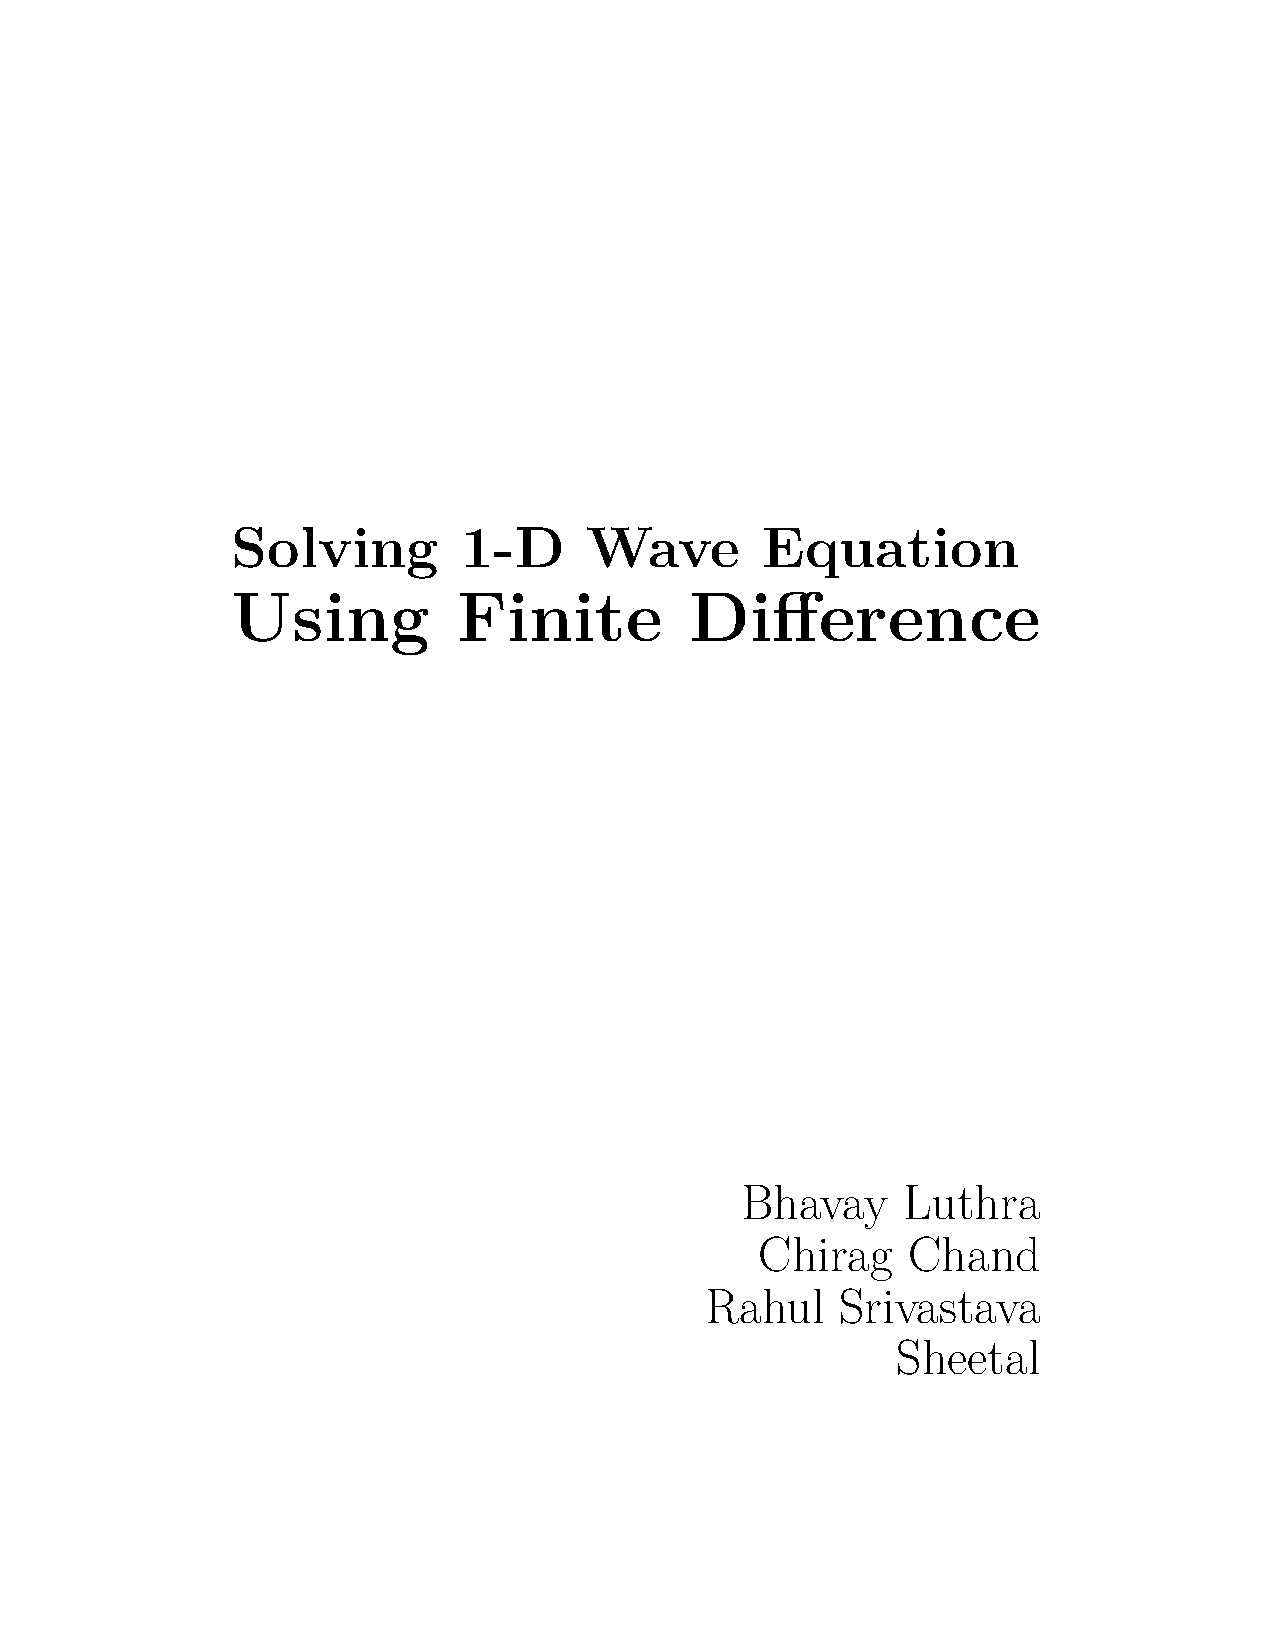
\includepdf[pages={1}]{Project.pdf}
        \tableofcontents
        \parindent=0pt
        \parskip=3pt
        
        \chapter{Introduction}

        In this article, we focus on the simple one-dimensional Wave Equation. 
        We show how the equation can be solved using the finite difference method. 
        We illustrate this by showing two solutions of the wave equation, a standing wave and a Gaussian pulse
        .By changing the general fortran formula , 
        the code can also be applied to other fundamental 
        one-dimensional equations such as Heat equation, and the Schrodinger equation.

  
                \section{Wave Equation}
                The wave equation is a second-order linear partial differential equation for 
                the description of waves—as they occur in classical physics—such as mechanical 
                waves (e.g. water waves, sound waves and seismic waves) or electromagnetic waves
                 (including light waves). It arises in fields like acoustics, electromagnetism, 
                 and fluid dynamics.\\ The scalar wave equation is:
                  
                $${\displaystyle {\frac {\partial ^{2}u}{\partial t^{2}}}\;=\;c^{2}\left({\frac {\partial ^{2}u}{\partial x_{1}^{2}}}+{\frac {\partial ^{2}u}{\partial x_{2}^{2}}}+\cdots +{\frac {\partial ^{2}u}{\partial x_{n}^{2}}}\right)}$$
                 
              where c is a fixed non-negative real coefficient which describes the speed of the wave.\\
              Using the notations of Newtonian mechanics and vector calculus, the wave equation can be written more compactly as:

              $${\displaystyle {\ddot {u}}=c^{2}\nabla ^{2}u}$$

                



 
                \section{Finite difference method}
                In numerical analysis, finite-difference methods (FDM) are a class of numerical techniques for solving differential equations by approximating derivatives with finite differences. Both the spatial domain and time interval (if applicable) are discretized, or broken into a finite number of steps, and the value of the solution at these discrete points is approximated by solving algebraic equations containing finite differences and values from nearby points.

                Finite difference methods convert ordinary differential equations (ODE) or
                 partial differential equations (PDE), which may be nonlinear, into a system of
                linear equations that can be solved by matrix algebra techniques. Modern 
                computers can perform these linear algebra computations efficiently which,
                  along with their relative ease of implementation, has led to the widespread
                 use of FDM in modern numerical analysis. Today, FDM are one of the 
                 most common approaches to the numerical solution of PDE, along with 
                  finite element methods.
 
        \chapter{Wave Equation}
        Waves are everywhere. A plethora of physical phenomena can be thought of as waves. And we are not talking about the water waves we all created when we were kids by throwing rocks in the lakes — although these were pretty cool —. Light, for example, is an electromagnetic wave propagating through space Sound is also an 
        example of a mechanical wave and, in particular, a pressure wave.
                \section{Waves in physics}
                Before we dive into the intricacies of the math behind the behavior
                 of waves let's begin by asking ourselves a simpler question.\emph{What is a wave?}\\
                \begin{align*}
                \begin{tabular}{|p{10cm}}
                \emph{In physics, a wave is a propagating disturbance of one or more quantities that travels through a medium from one location to another. Wave motion transfers energy from one point to another, usually without permanent displacement of the particles of the medium.}
                \end{tabular}\\
                \end{align*}

                Mechanical waves, such as sound, require a medium through which to travel, 
                while electromagnetic waves do not require a medium and can be propagated
                 through a vacuum. Propagation of a wave through a medium depends on the medium's 
                 properties. Based on that, the speed at which a wave travels depends solely on
                  the medium itself and not on the wave at all! It does not matter how hard or 
                  soft or at what angle you throw a rock in a lake. 
                The waves will spread out at exactly the same speed.
                \href{https://imgur.com/x7cjP8r}{\underline{A transverse wave propagating in a string/rope}}\\               
                \begin{figure}[hbtp]
                        \caption{Particle movement is perpendicular to the propagation in a transverse wave}
                        \hspace*{3cm}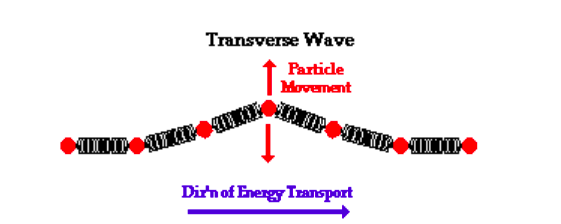
\includegraphics[scale=0.5]{trans.png}        
                \end{figure}

                A longitudinal wave is a wave in which particles of the medium 
                move in a direction parallel to the direction that the wave moves. 
                An example of a longitudinal wave is a wave on a slinky as shown below.
                \href{https://imgur.com/qAsFFSb}{\underline{A longitudinal wave propagating in a slinky}}\\
                \begin{figure}[hbtp]
                        \caption{Particle movement is parallel to the propagation in a longitudinal wave}
                        \hspace*{3cm}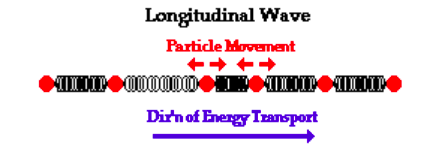
\includegraphics[scale=0.5]{longitudnal.png}
                \end{figure}

                Finally, when two waves moving in opposite directions, 
                having the same amplitude and frequency, 
                are combined we get a standing wave — also known as a stationary wave :

                \href{https://imgur.com/EEuwsY9}{\underline{A standing wave (black) as a result of two ways moving in opposite directions (red and blue)}}\\

                Okay, we now know some of the fundamental ideas 
                regarding waves in physics. We are ready to dive 
                into the mathematics behind the equation that 
                describes the behavior of any wave known as the 
                wave equation.



                \section{The Wave Equation}
                        The one-dimensional equation that describes 
                        how any kind of disturbance propagates through
                         a medium i.e. the wave equation is the following:

                        $${\displaystyle {\frac {\partial ^{2}u}{\partial t^{2}}}=c^{2}{\frac {\partial ^{2}u}{\partial x^{2}}}.}$$
                        where $\mathbf{u = u(x,t)}$ is the displacement of the
                        particle of the wave located at position x at time t and c 
                        is the speed at which the wave is propagating.\\


                        We will not present a formal mathematical proof of the
                        aforementioned equation in this project.
                        Instead, we will try to present an intuitive interpretation of what it represents. Let's begin!

 
                \section{Developing Intuition}                
                Suppose that two friends, Alice and Bob are 
                playing with a string. Alice is holding one end of 
                the string while Bob is holding the other. They are
                 both moving their hands up down trying to create 
                 some sort of wave in that string.\\
                 \begin{figure}[hbtp]
                        \caption{Bob and Alice playing with a string}                        
                        \hspace*{2cm}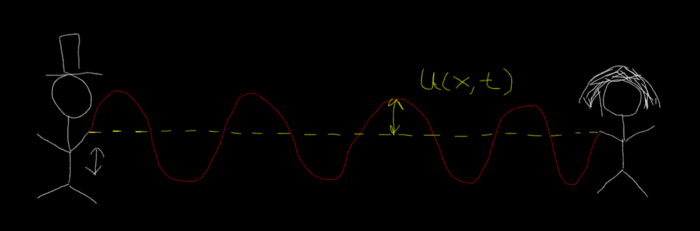
\includegraphics[scale=0.5]{a&b_1.png}
                \end{figure}\\
                We now take our binoculars and we zoom in in that 
                string trying to figure out what exactly is going on.
                Bob and Alice create a wave with their hand motion which propagates 
                through the string. In order for that to happen, a force must be 
                exerted to the particles of the string which constantly move up 
                and down. That force is tension.\\
                \begin{figure}[hbtp]
                        \caption{An element of the string}                        
                        \hspace*{2cm}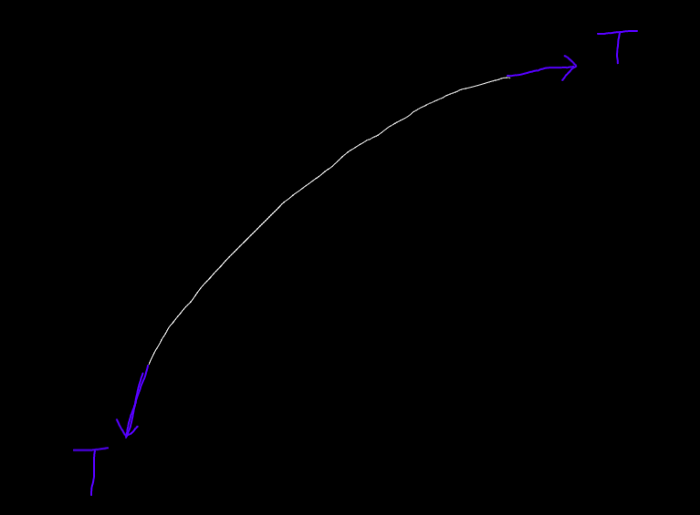
\includegraphics[scale=0.5]{a&b_2.png}
                \end{figure}\\

                The tension acts tangent to the direction of the 
                string it pulls the string apart as seen in the image above. 
                For simplicity purposes, we will assume that the tension is
                 constant throughout the string — which can be easily proven
                  for small disturbances .\\

                Now, notice that the part of the string that we 
                zoomed in is curved downwards. 
                The vertical components of both of the tensions at
                 the end of the string can be seen in the image below.
                 \begin{figure}[hbtp]                        
                        \hspace*{4cm}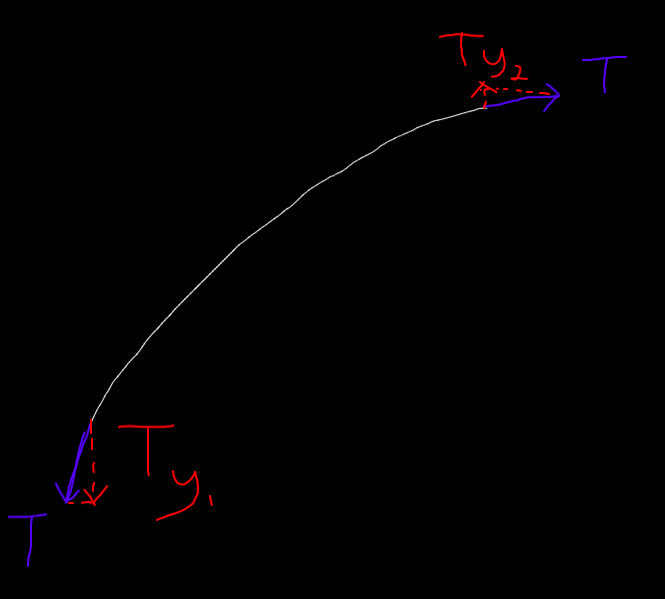
\includegraphics[scale=0.3]{a&b_3.png}
                \end{figure}\\

                It is obvious that $Ty_1 > Ty_2$ and thus, the net tension 
                force is directed downwards. On the other hand, if we had 
                zoomed in on another element of the string that was curved the other way, 
                the net vertical tension would be directed upwards.
                \begin{figure}[hbtp]
                        \caption{$Ty_1 > Ty_2$ The net vertical tension is directed upwards}                        
                        \hspace*{2cm}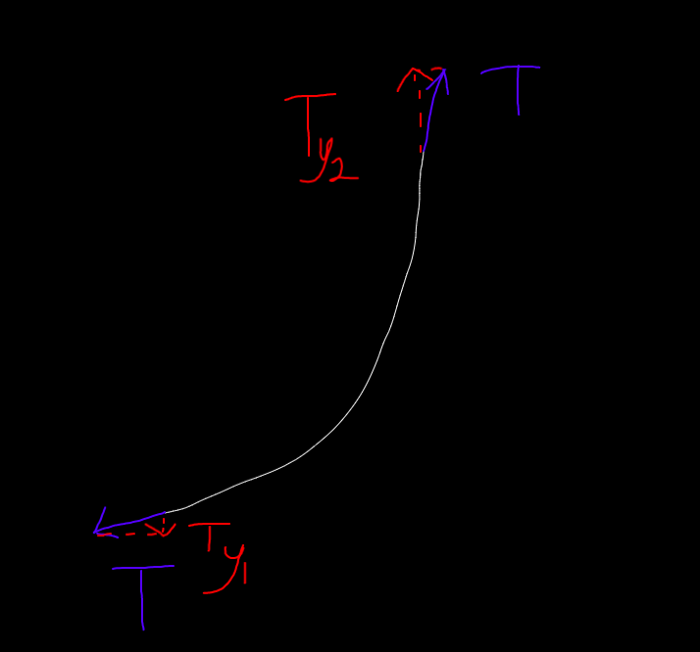
\includegraphics[scale=0.5]{a&b_4.png}
                \end{figure}\\

                \textcolor{red}{We can conclude that the concavity of 
                the string i.e. the way it is curved is 
                related to the net tension applied to the string.}\\
                
                As we know from calculus, the concavity 
                of a function is indicated by the sign of
                 its second derivative. If the function's 
                 second derivative is positive, the graph 
                  concaved up while if it's negative, the graph
                 is concaved down.
                 \begin{figure}[hbtp]
                        \caption{Concavity of a function f = f(x)}                        
                        \hspace*{2cm}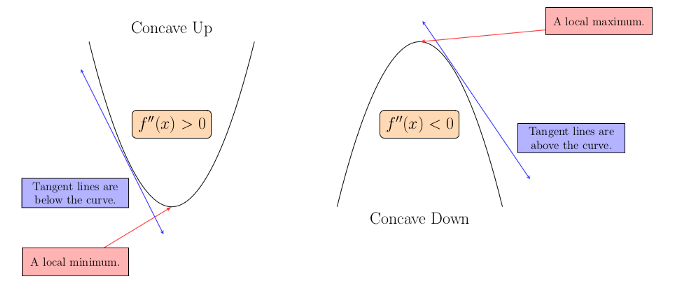
\includegraphics[scale=0.5]{concave.png}
                \end{figure}\\
                From Newton's second law, we can relate the net vertical
                tension to the acceleration of the string i.e. 
                the second time derivative of its vertical displacement

                $$\Sigma F=ma=m\frac{d^2u}{dt^2}$$
                With all this in mind, it is evident that 
                the second spatial derivative of the vertical 
                displacement of the string is related to its second 
                time derivative. To summarize:
                \begin{figure}[hbtp]
                        \caption{}                        
                        \hspace*{4cm}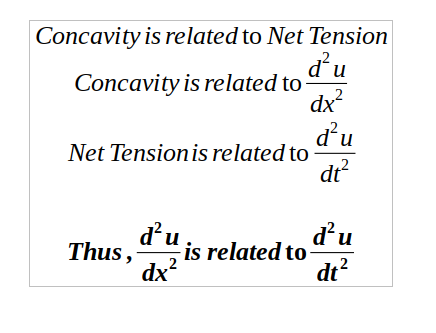
\includegraphics[scale=0.5]{summary.png}
                \end{figure}\\
                It can be easily proven mathematically that not
                 only are these two quantities related but they
                  are proportional to each other. If we name the 
                  proportionality constant c² then we arrive at the
                   wave equation!

                \section{Solution}

                If we now perform some factorization 
                in the wave equation we can reach the following form:

                $$\frac{d^2u}{dt^2}=c^2\frac{d^2u}{dx^2}\rightarrow c^2\frac{d^2u}{dx^2}-\frac{d^2u}{dt^2}=0\rightarrow (c\frac{du}{dx}-\frac{du}{dt})(c\frac{du}{dx}+\frac{du}{dt})=0$$

                We can see that $u(x, t) = u(x - ct)$ and $u(x, t) = u(x+ct)$ are solutions respectively. The point here is that the wave equation 
                describes any disturbance that has a left and 
                right component. Since c is positive, the term
                $x - ct$ becomes smaller as time passes while $x+ct$ 
                becomes larger.\\

                Thus, whatever u describes, the term $u(x - ct)$ corresponds
                 to a disturbance moving to the right while the 
                 term $u(x+ct)$ corresponds to one moving to the left.
                Thus, the equation for a standing wave can easily be
                 produced by adding two solutions moving in opposite
                  directions $u = u(x -ct) + u(x+ct)$  which have the same amplitude
                   and frequency.


 
        \chapter{Finite Difference Method}
        To solve the 1-D wave equation we have a couple of methods like Method of lines , Finite element method, Gradient discretization method , etc
        but in this docment we will be using the Finite difference method solve out 1-D wave equation.\\
        In this method, functions are represented by their values at certain grid points and derivatives are approximated through differences in these values.

        
                \section{Finite Difference Method}
                This method use the neat property of Taylor ploynomial to calculate the derivate of a function by using taylor series. 
                Thus we can calculate the nth order deivate with n intial condition.\\

                Recall that the derivative of a function was defined by taking the limit of a difference quotient:
                        $$f'(a)=\lim _{h\to 0}{\frac {f(a+h)-f(a)}{h}}\rightarrow (8.1)$$
                        Now to use the computer to solve differential equations we go in the opposite direction - we replace derivatives
                        by appropriate difference quotients. If we assume that the function can be differentiated many times then Taylor's
                        Theorem is a very useful device to determine the appropriate difference quotient to use. For example, consider:
                $$ f(x_0 + h) = f(x_0) + \frac{f'(x_0)}{1!}h + \frac{f^{(2)}(x_0)}{2!}h^2 + \cdots + \frac{f^{(n)}(x_0)}{n!}h^n + R_n(x) \rightarrow (8.2)$$       
                Re-arranging terms in (8.2) and dividing by $\Delta x$ we obtain:
                $${f(a+h)\over h} = {f(a)\over h} + f'(a)+{R_1(x)\over h} $$
                Solving for $f'(a)$:
                $$f'(a) = {f(a+h)-f(a)\over h} - {R_1(x)\over h}$$
                ssuming that ${\displaystyle R_{1}(x)}R_1(x)$ is sufficiently small, the
                 approximation of the first derivative of "f" is:
                $$f'(a)\approx {f(a+h)-f(a)\over h}$$
                This is, not coincidentally, similar to the definition of derivative (eqn 8.1).

                \section{1-D Wave Equation using FDM}
                First we define the $\mathbf{\text{Shortcut Notation}}$:
                $$u_t=\frac{\partial u}{\partial t}$$
                $$u_{xx}=\frac{\partial^2 u}{\partial x^2}$$
                Then our 1-D wave equation can be written as :
                $$u_{tt}=c^2 u_{xx}$$
                \subsection{Formulae Used}
                \begin{enumerate}
                        \item First Derivates:
                \begin{align*}
                                 \text{Forward Difference} &: f'(x)\approx\lim_{\Delta x\to 0}\frac {f(x+\Delta x)-f(x)}{\Delta x}\\
                                \text{Backward Difference} &: f'(x)\approx\lim_{\Delta x\to 0}\frac {f(x)-f(x+\Delta x)}{\Delta x}\\
                                 \text{Central Difference} &: f'(x)\approx\lim_{\Delta x\to 0}\frac {f(x+\Delta x)-f(x-\Delta x)}{\Delta x}\\
                \end{align*}
                        \item   Second Derivates:
                        \begin{align*}
                                \text{Central Difference} &: f''(x)\approx\lim_{\Delta x\to 0}\frac {f(x+\Delta x)-f(x)+f(x-\Delta x)}{2\Delta x}                             
                        \end{align*}
               
                        \item First Order  Derivates:
                \begin{align*}
                                 \text{Forward Difference} &: u_t(x,t)\approx\lim_{\Delta t\to 0}\frac {u(x,t+\Delta t)-u(x,t)}{\Delta t}\\
                                \text{Backward Difference} &: u_x(x,t)\approx\lim_{\Delta x\to 0}\frac {u(x,t)-u(x-\Delta x,t)}{\Delta x}\\
                                 \text{Central Difference} &: u_t(x,t)\approx\lim_{\Delta t\to 0}\frac {u(x,t+\Delta t)-u(x,t-\Delta t)}{2\Delta t}\\
                \end{align*}
                        \item   Second Order Derivates:
                        \begin{align*}
                                  \text{Central Difference} &: u_t(x,t)\approx\lim_{\Delta t\to 0}\frac {u(x,t+\Delta t)-2u(x,t)+u(x,t-\Delta t)}{(\Delta t)^2}\\ 
                                                                  &: u_t(x,t)\approx\lim_{\Delta x\to 0}\frac {u(x+\Delta x,t)-2u(x,t)+u(x-\Delta x,t)}{(\Delta x)^2}                            
                        \end{align*}
                \end{enumerate} 
                \section{Boundary \& Initial Conditions}
                \begin{center}
                \begin{itemize}
                        \item $u_{tt}=c^2u_{xx}$  $0<x<L$
                        \item Boundary Conditions :$ u(0,t)=0$ , $u(L,t)=0$
                        \item Initial Conditions: $u(x,0)=f(x)$ , $u_t(x,0)=g(x)$
                \end{itemize}        
                \end{center}
                \subsection{Solving}
                $$u_{tt}=c^2u_{xx}$$
                $$x_{i+1}=x_i+\Delta x$$
                $$t_{j+1}=t_j+\Delta t$$
                $$\frac{u(x_{i},t_{j+1})-2u(x_i,t_j)+u(x_i,t_{j-1})}{(\Delta t)^2}=c^2 \frac {u(x_{i+1},t_j)-2u(x_i,t_j)+u(x_{i-1},t_j)}{(\Delta x)^2}$$
                $$u(x_i,t_{j+1}) = 2y(x_i,t_j) +  \lambda*(y(x_{i+1},t_j)-2y(x_i,t_j) + y(x_{i-1},t_j)) - y(x_i,t_{j-1})$$
                $$\text{here:} \hspace*{5pt} \lambda=c^2\frac{\Delta t^2}{\Delta x^2}$$
                
        \chapter{Standing Wave}
        In physics, a standing wave, also known as a stationary wave, is a wave that oscillates in time but whose peak 
        amplitude profile does not move in space. The peak amplitude of the wave oscillations at any point in space is 
        constant with respect to time, and the oscillations at different points throughout the wave are in phase. The locations at which the absolute value of the amplitude is
         minimum are called nodes, and the locations where the absolute value of the amplitude is maximum are called antinodes.\\
        
        General Equation :
                 
                $${\displaystyle y(x,t)=2y_{\text{max}}\sin \left({2\pi x \over \lambda }\right)\cos(\omega t)}$$
                \begin{figure}[hbtp]
                        \caption{For the fundamental frequency of a standing wave between two fixed ends, the wavelength is double the length of the string.}
                        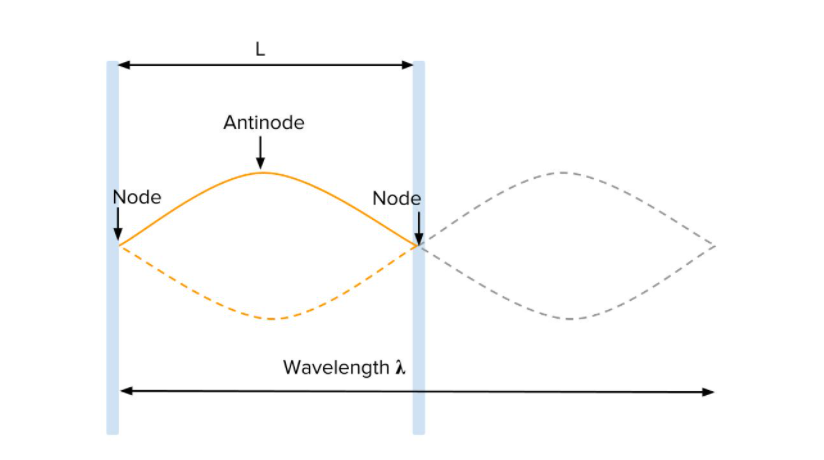
\includegraphics[scale=0.9]{standing_wave.png}        
                \end{figure}
                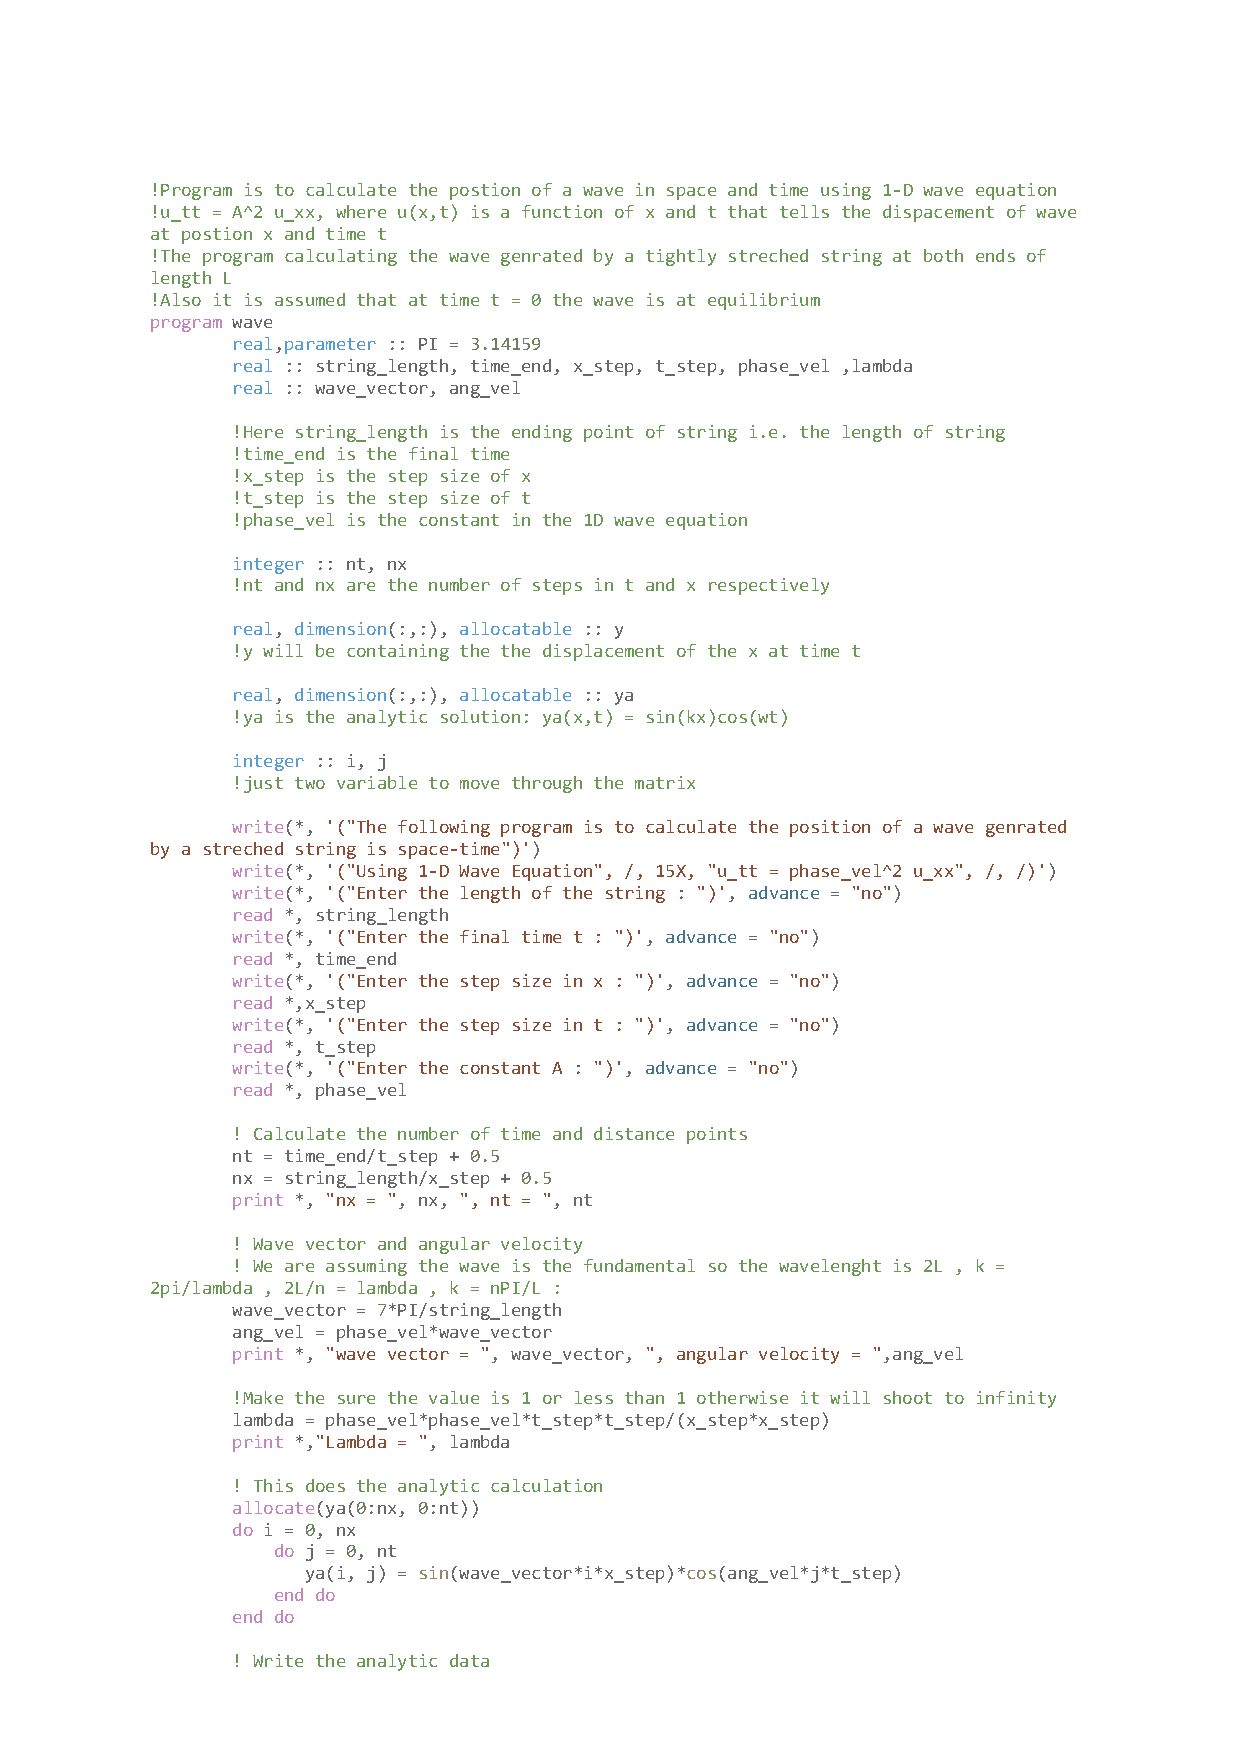
\includepdf[pages=1,pagecommand=\section{Fortran Code},offset=0 -1cm]{wave_standing.pdf}
                \includepdf[pages=2-]{wave_standing.pdf}


                \section{Gnu script}
                \begin{figure}[hbtp]
                        \caption{Snapshot of the GNU Script}
                        \hspace*{1cm}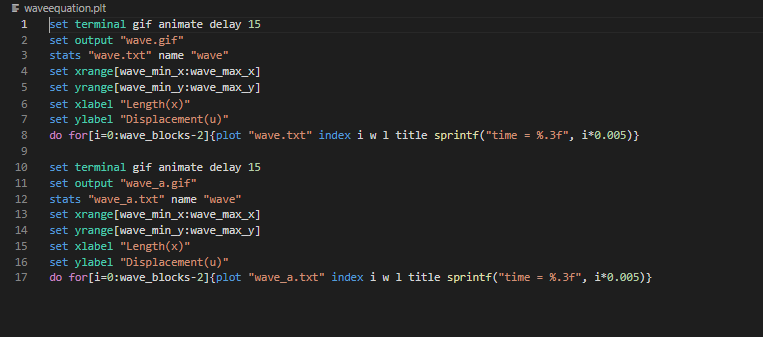
\includegraphics[scale=0.7]{wave_gnu.png}        
                \end{figure}
                The first para creates the file wave.gif which is generated from the points in the wave.txt. This is the numerical
                solution.\\
                The Second para  creates the file wave\_a.gif which is generated from the points in the wave\_a.gif . This is the analytical
                solution.
                \section{Ouputs}
                        \subsection{Analytical \& Numerical}
                        We first run the fortran code to generate the text file.
                        Input as follows:
                        \begin{figure}[hbtp]
                                \caption{Input for the fortran code}
                                \hspace*{1cm}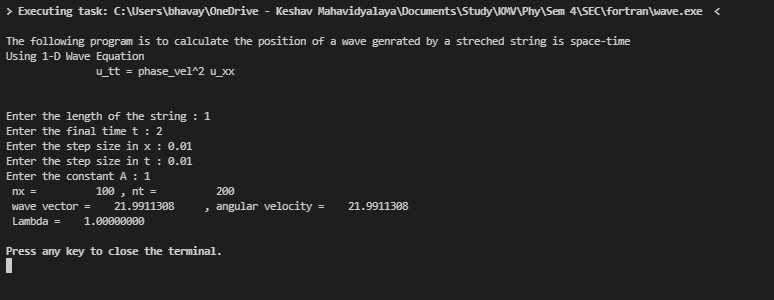
\includegraphics[scale=0.7]{wave_fortran.png}        
                        \end{figure}\\
                        Next we run the gnu script file to create the two gif files. To look at the actual solution , I have uploaded 
                        the gif files on imgur. Here , I only will be post the stills from the two gif.\\
                        \begin{figure}[hbtp]
                                \caption{Still from the Numerical solution}
                                \hspace*{3cm}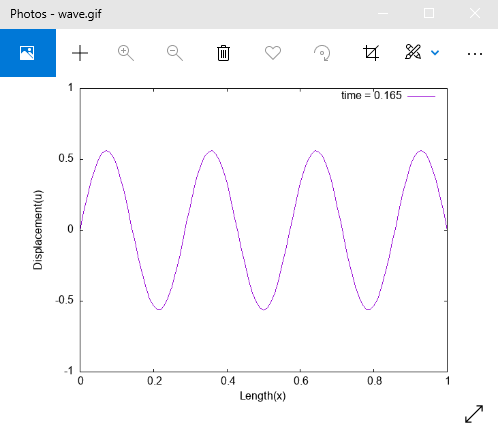
\includegraphics[scale=0.7]{wave_numerical.png}        
                        \end{figure}
                        \pagebreak
                        \begin{figure}[hbtp]
                                \caption{Still from the analytical solution}
                                \hspace*{3cm}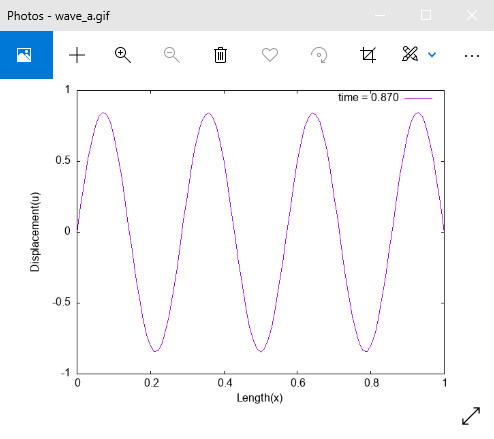
\includegraphics[scale=0.7]{wave_analytical.png}        
                        \end{figure}\\
                        Here is the link for the actual gifs:\\
                        \href{https://imgur.com/a/AoAPeOX}{\underline{Analytical Solution}}\\
                        \href{https://imgur.com/a/WHFYH6b}{\underline{Numerical Solution}}\\[5pt]

                        \textcolor{red}{BONUS!!}\\
                        I also uploaded the text file on the google drive which is generated from running fortran code.\\
                        \href{https://drive.google.com/file/d/1kXk8Ap_GSktrb_hs_hzjusJ-BBUGSaDM/view?usp=sharing}{\underline{Analytical Solution}}\\
                        \href{https://drive.google.com/file/d/1Afp1AZzLBLb2BL8miCo2TCGyx1rZjwZ7/view?usp=sharing}{\underline{Numerical Solution}}
                        \chapter{Pulse Wave}
                        In chapter 4 we discussed using the wave equation to model a standing wave. This is a particularly simple solution since the standing wave is formed from a single sinusoidal wave reflected from the ends of the string, and it admits a simple analytical solution that can be compared with the numerical calculation. However we can use the finite difference method to calculate the time evolution of more complex waves, and to illustrate this in this chapter we consider a Gaussian pulse moving along the string. This will be familiar to many of us as the wave we observe when flicking the end of a rope.

                        \begin{figure}[hbtp]
                                \caption{ Plot of a harmonic wave at t = 0 and t = $\Delta$t.}
                                \hspace*{2cm}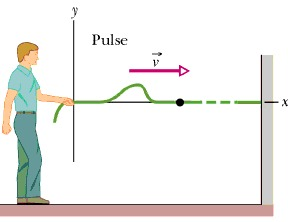
\includegraphics[scale=0.9]{travelling_wave(1).png}        
                        \end{figure}

The equation for the pulse is:

$$ y(x,t) = A \exp(-(x - vt)^2/a^2) $$

where $A$ is the peak amplitude, $v$ the wave velocity and $a$ a constant that describes the pulse width. This pulse moves in the positive $x$ direction at velocity $v$.

For the numerical solution we need only change the initial conditions. We set $y(x,0)$ and $y(x,dt)$, where $dt$ is the time increment, using the equation above, and as before the ends of the string are clamped so the wave reflects from them. The code is given in the first part of section 5.1.

This time the analytic solution is more complex as we need to reflect the wave from the ends of the string and sum the incident and reflected pulses. Due to this added complexity the analytic solution has been done in a separate program given in the second part of section 5.1.

Sections 5.3 onwards give the results and associated discussion.

                          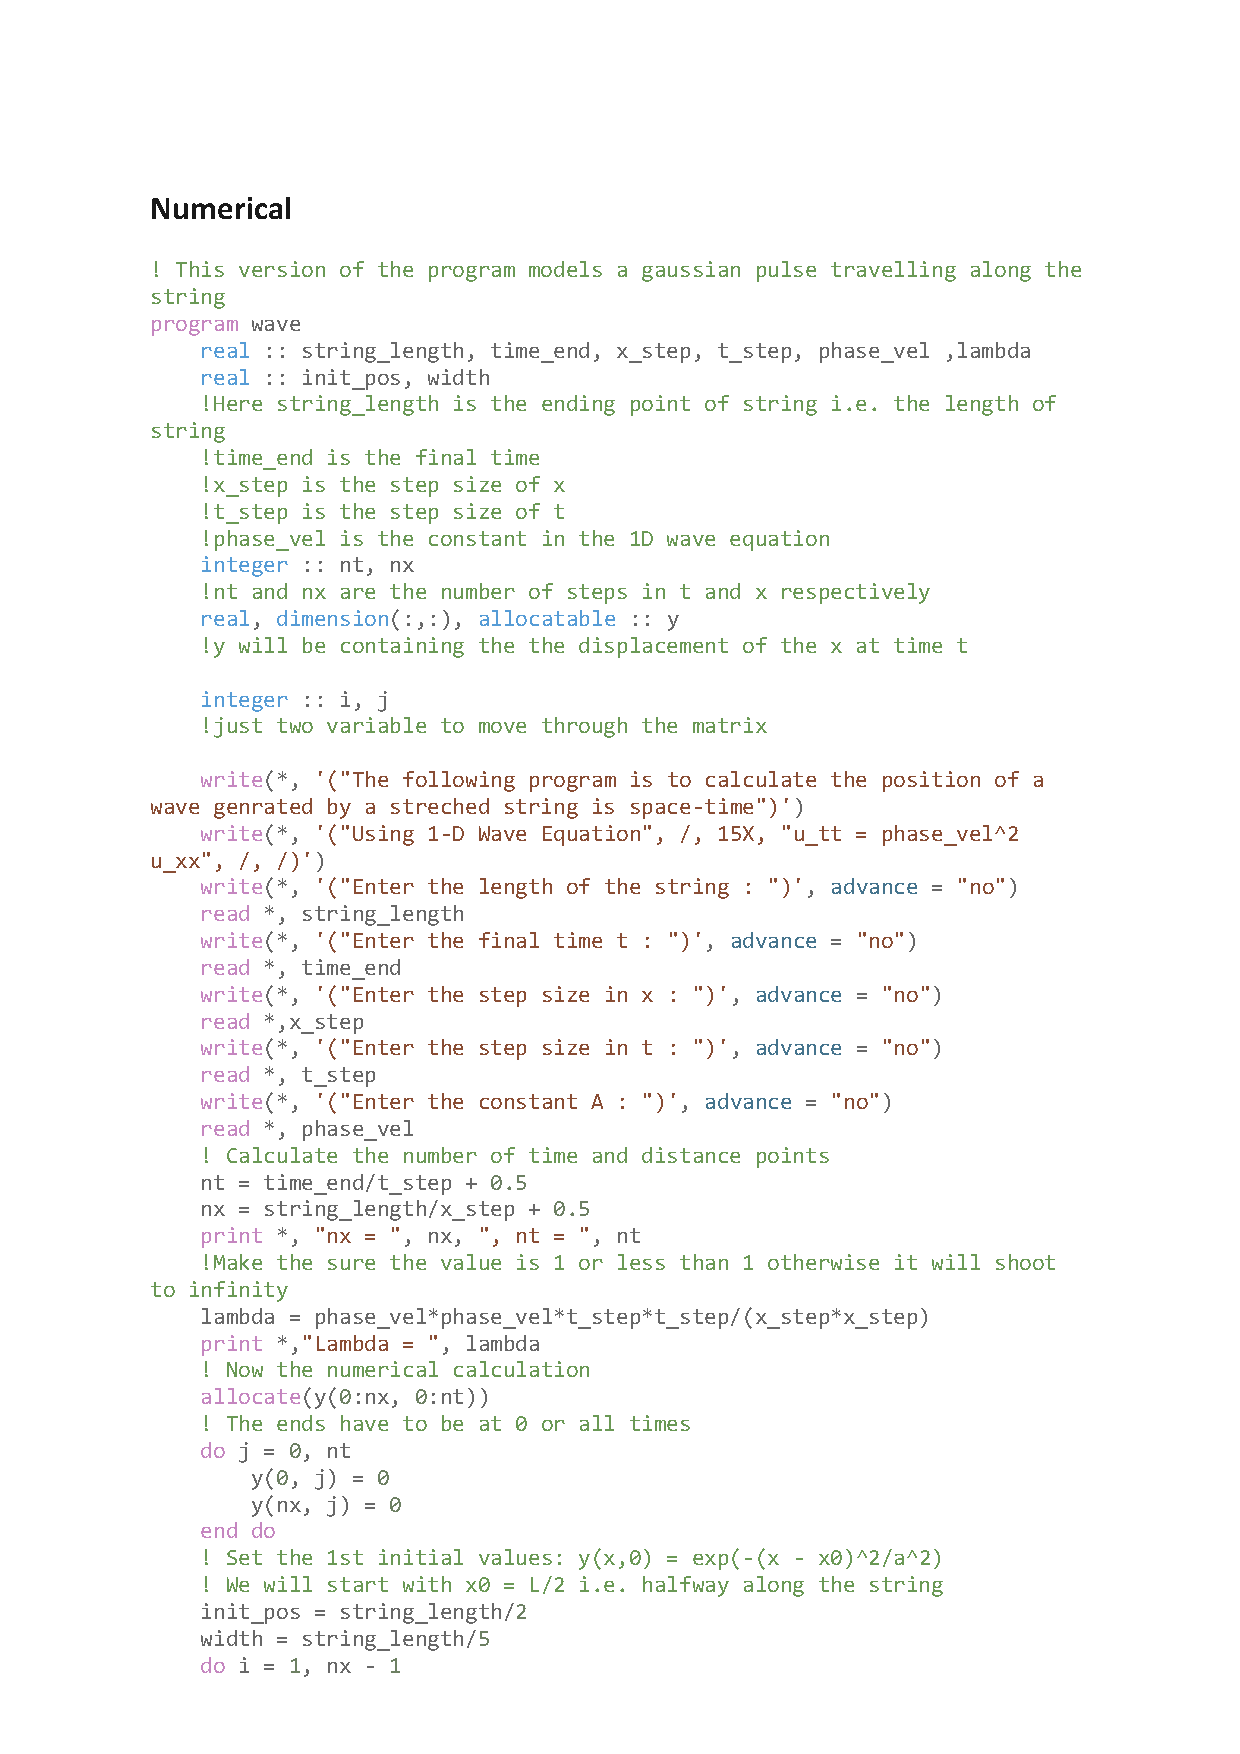
\includepdf[pages=1,pagecommand=\section{Fortran Code},offset=0 -2cm,scale=.9]{wavepulse_5.pdf}
                          \includepdf[pages=2-]{wavepulse_5.pdf}
                                 
                                       
                                \section{GNU Script}
                                \subsection{Analytical}
                                \phantom{a}
                                \begin{figure}[hbtp]
                                        \caption{Snapshot of the GNU Script (Analytical)}
                                        \hspace*{1cm}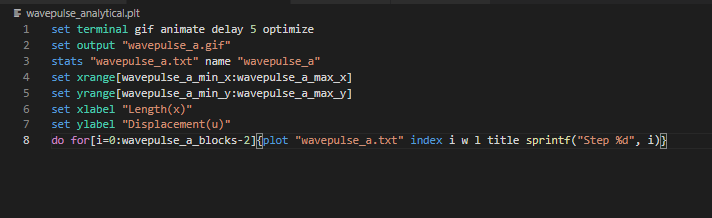
\includegraphics[scale=0.7]{wavepulse_gnu_analytical.png}        
                                \end{figure}
                                \subsection{Numerical}
                                \begin{figure}[hbtp]
                                        \caption{Snapshot of the GNU Script (Numerical)}
                                        \hspace*{1cm}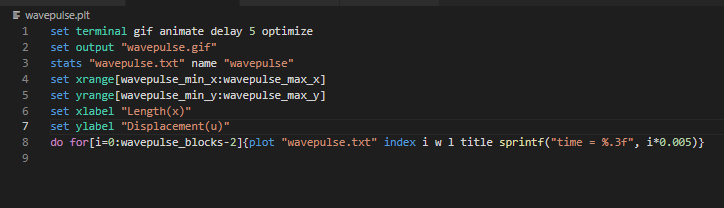
\includegraphics[scale=0.7]{wavepulse_gnu_numerical.png}        
                                \end{figure}
                                \section{Output}
                                We first run the fortran code to generate the text file. 
                                Input as follows:\\
                                \begin{figure}[hbtp]
                                        \caption{Input for the fortran code}
                                        \hspace*{3cm}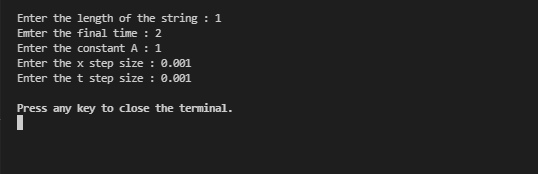
\includegraphics[scale=0.7]{wavepulse_fortran.png}        
                                \end{figure}\\
                                Next we run the gnu script file to create the two gif files. To look at the actual solution , I have uploaded 
                                the gif files on imgur. Here , I only will be post the stills from the two gif.
                                \begin{figure}[hbtp]
                                        \caption{Still from the Numerical solution}
                                        \hspace*{3cm}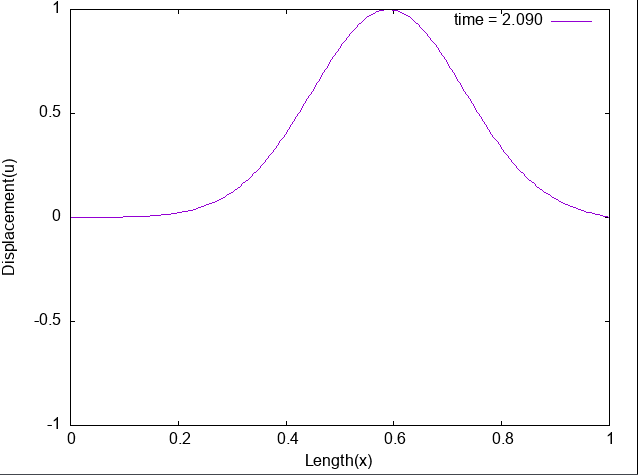
\includegraphics[scale=0.6]{wavepulse_still_numerical.png}        
                                \end{figure}
                                \begin{figure}[hbtp]
                                        \caption{Still from the analytical solution}
                                        \hspace*{3cm}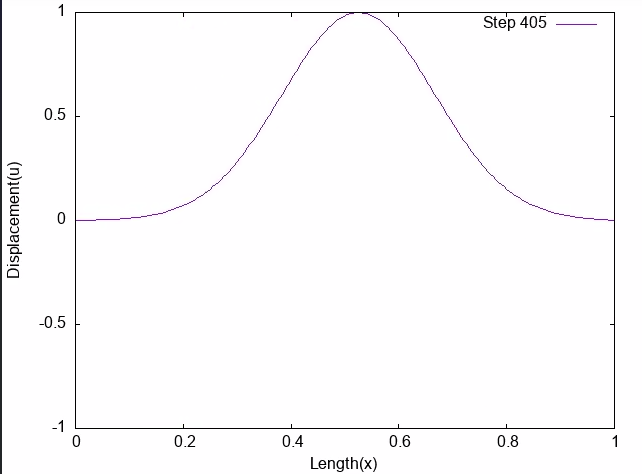
\includegraphics[scale=0.6]{wavepulse_still_analytical.png}        
                                \end{figure}
                                
                                Here is the link for the actual gifs:\\
                                \href{https://imgur.com/a/iwEF6XL}{\underline{Analytical Solution}}\\
                                \href{https://imgur.com/a/kZL1kjg}{\underline{Numerical Solution}}\\[5pt]

                                \textcolor{red}{BONUS!!}\\
                                I also uploaded the text file on the google drive which is generated from running fortran code.\\
                                \href{https://drive.google.com/file/d/1bfo3J55lOWPwkmFMmFRtC1iScOuUE_pA/view?usp=sharing}{\underline{Analytical Solution}}\\
                                \href{https://drive.google.com/file/d/1Afp1AZzLBLb2BL8miCo2TCGyx1rZjwZ7/view?usp=sharing}{\underline{Numerical Solution}}
                  
\end{document}